\chapter{Assignment 3: Alternative Splicing}

When scientists first mapped human DNA, they found something very surprising. 
For a long time, the rule in biology was simple: one gene makes one protein. Based on this, people thought humans would have a huge number of genes because we are a very complex species. 

However, it turns out we have about 20,000 to 25,000 genes. This is almost the same number of genes as a tiny, simple worm. 
The main answer is a process called alternative splicing \cite{wang2015mechanism, stamm2005function}.

For the understanding of what it is Alternative Splicing, we can somehow think of a gene as a set of draft instructions. When the cell reads a gene, it first makes a temporary copy. 
This copy contains two types of pieces. There are the useful pieces. 
Then there are the blank or "junk" pieces in between. 

Before the cell can use these instructions to build a protein, it has to clean them up. A special machine inside the cell cuts out all the blank pieces and glues the useful pieces together. 

This cleanup process is called splicing \cite{wang2015mechanism}.

\begin{figure}[h]
    \centering
    \includegraphics[width=\linewidth]{./assets/Alternative splicing.png} 
    \caption{Diagram that repersents the alternative splicing process.}
    \label{fig:exon_skipping}
\end{figure}

Alternative splicing is what happens when the cell gets a little bit more creative. 
Instead of always gluing all the useful pieces together in the exact same way every time, the cell can change the pattern.

Sometimes it might skip a useful piece. Other times it might keep a part of a blank piece. Because of this, that single original set of draft instructions can be used to make many different final instruction manuals.
This means one single gene can produce many different types of proteins, each doing a slightly different job \cite{wang2015mechanism, stamm2005function}.

This process is a big part of how animals became more complex over millions of years. As life evolved from simple single cells to complex animals, the actual number of genes did not grow very fast. 
Instead, nature used alternative splicing to get more variety out of the genes that were already there \cite{ast2004evolve}. 

Over a very long time, some of the blank, unused parts of the DNA slowly changed. They turned into new useful pieces \cite{ast2008bioessays, ast2004evolve}.

\begin{figure*}[t]
    \centering
    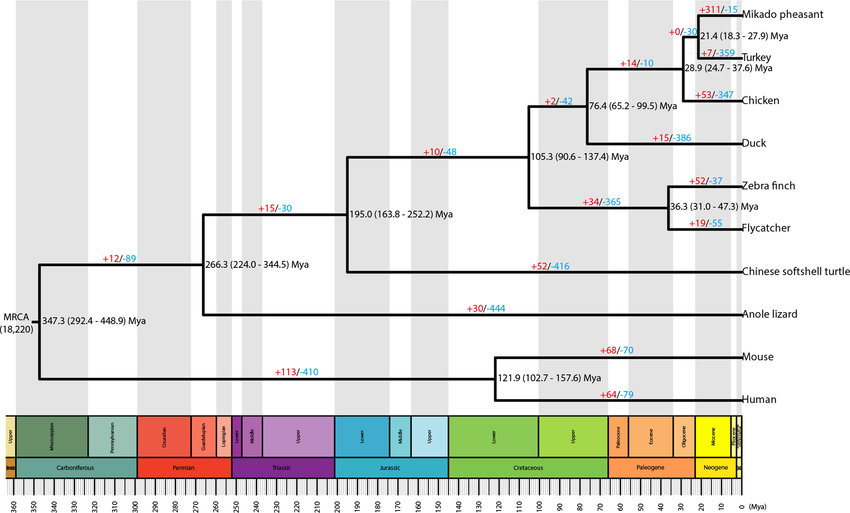
\includegraphics[width=0.75\textwidth]{./assets/Evolution-of-gene-families-among-various-animal-species-A-phylogenetic-tree-was-414748790.jpg} 
    \caption{Evolutionary expansion of gene families in animals.}
    \label{fig:evolutionary_expansion}
\end{figure*}

There is also a reason why humans and other complex animals use this trick more than simple organisms. In simple life forms, the blank spaces are very short. The cell's machinery focuses on finding these short blank spaces to cut them out. But in humans, the blank spaces are incredibly long, and the useful pieces are very short. Because of this, our cells changed their strategy. 
The machinery looks for the short useful pieces instead of the long blank spaces. When the machine is looking for small pieces in a huge sea of blank space, it is much easier to just accidentally or purposefully skip one. This makes our genes naturally ready for alternative splicing \cite{ast2008bioessays}.

This ability to mix and match is very important for our survival. Different parts of our body need different things. The cells in our brain need different proteins than the cells in our immune system. Alternative splicing allows the body to use the exact same genes but customize the final proteins for each specific body part \cite{marasco2023physiology, stamm2005function}. 